\chapter{Shadowing Experiments with Natural and Synthetic Voices}
\label{chap:shadowing_experiment_with_natural_and_synthetic_voices}

\lettrine{A} series of experiments is described in this chapter.
Some of them were designed to determine human behavior in \acl{hhi} and \ac{hci} as a mean of modeling interactions, and others examined the change in reactions of subjects to different adaptation strategies of implemented system as a subjective evaluation method.

\pagebreak

\section{Convergence to natural and synthetic stimuli}
\label{sec:convergence_to_natural_and_synthetic_stimuli}

something\ldots

\subsection{Design}
\label{subsec:design_HCIConv}

\subsubsection{Target features}
\label{subsec:target_features_HCIConv}

\todo{little intro}

\begin{enumerate}    
	\item \textbf{\textipa{[\c{c}]} vs.\ \textipa{[k]} at a word-final $\langle$-\textit{ig}$\rangle$} syllable
	
	These variations of the phoneme \textipa{[\c{c}]} are both common native speakers of German.
	Using one variation or the other does not change the meaning of the word, or any other property of it.
	Although it can be generally said that \textipa{[\c{c}]} is more used in the south and \textipa{[k]} in the north of Germany, they do not mark a specific dialect or socio-economic status.
	This \enquote{neutrality} makes this feature a good candidate, since change in pronunciation should not occur due to the liking of one dialect or the other, or as an attempt to match a certain social status.
	It is noteworthy that the \textipa{[\c{c}]} variation is considered to be more standard, but still, both of the variations are accepted and people typically do not even notice which variation they and their interlocutors are using.
	In this experiment, we treat this feature as bi-categorical in nature.
	The very few instances of other fricatives (such as \textipa{[S]} and \textipa{[J]}) were counted as \textipa{[\c{c}]} as well, making the distinction practically between fricative and plosive realization.
	Here are two examples of sentences with this features that were used as material for the experiment's stimuli (for the full list of stimulus materials, see \autoref{app:shadow_experiment_stimul}):
	
	\begin{enumerate}[label=\arabic{enumi}\alph*), ref=\arabic{enumi}\alph*.)]
		\item 
		\begin{tabulary}{\linewidth}{LLL}
			Der & köni\textbf{\underline{g}} & hält eine Rede.\\
			\textit{The} & \textit{king} & \textit{spoke}.\\
		\end{tabulary}
		\item
		\begin{tabulary}{\linewidth}{LLLLL}
			Ich & bin & süchti\textbf{\underline{g}} & nach & Schokolade.\\
			\textit{I} & \textit{am} & \textit{addicted} & \textit{to} & \textit{chocolate}.\\
		\end{tabulary}
	\end{enumerate}
	
	\item \textbf{\textipa{[e:]} vs.\ \textipa{[E:]} realization of the mid-word grapheme \enquote{ä}}
	
	These two phonemes represent the two extremes of this feature's realization.
	However, vowel quality, as opposed to the \textipa{[\c{c}]} vs.\ \textipa{[k]} feature, it is not categorical (fricative vs.\ plosive), but rather gradual.
	That means that the actual realization can be anywhere between these two extremes.
	Despite the gradual nature of vowel quality, native speakers still perceive this feature as categorical (either \textipa{[e]} or \textipa{[E]}, cf.\ \citet{Kuhl2004early, Kuhl1991human}).
	\review{are these references relevant? is this really magnet effect?}
	In this experiment, we treat this feature as categorical in the first phase (see \cref{subsubsec:procedure_hci}), but measure it as gradual for analysis purposes (see \cref{subsec:results_hci}).
	This allows the detection of non-categorical changes over time, which are important for characterizing the convergence process.
	The \textipa{[E]} variation is in general more typical for the southern federal states of Germany, while \textipa{[e]} is more common in the north.
	As in the case of the \textipa{[\c{c}]} vs.\ \textipa{[k]} feature, the use of one realization or the other (or any in-between them) does not make any difference in meaning.
	Here are two examples of sentences with this features that were used as material for the experiment's stimuli (for the full list of stimulus materials, see \autoref{app:shadow_experiment_stimul}):
	
	\begin{enumerate}[label=\arabic{enumi}\alph*), ref=\arabic{enumi}\alph*.)]
		\item 
		\begin{tabulary}{\linewidth}{LLLLL}
			War & das & Ger\textbf{\underline{ä}}t & sehr & teuer?\\
			\textit{was} & \textit{the} & \textit{device} & \textit{very} & \textit{expensive}?\\
		\end{tabulary}
		\item
		\begin{tabulary}{\linewidth}{LLLLLL}
			Ich & mag & die & Qualit\textbf{\underline{ä}}t & deiner & Tasche.\\
			\textit{I} & \textit{like} & \textit{the} & \textit{quality} & \textit{of your} & \textit{bag}.\\
		\end{tabulary}
	\end{enumerate}
	
	\item \textbf{\textipa{[@n]} vs.\ \textipa{[\s{n}]} at a word final $\langle$-\textit{en}$\rangle$ syllable}
	Unlike the two previous features, this feature does not, typically, show variation in -- all the more so in spontaneous speech, which is more relevant in the context of \acp{sds}.
	While the \textipa{[@n]} variation may occur when one wants to emphasize the word/syllable or when speaking more clearly, e.g., with children or when in a noisy environment, the \textipa{[\s{n}]} variation is by a large margin the more dominant one.
	It is rare to hear consistent production of a \textipa{[@n]} in an ending-syllable $\langle$-\textit{en}$\rangle$.
	This is true across-dialects and regions, and it is ascribed to the phonological rule \textit{schwa epenthesis} that occurs in the German language, as follows (simplified version adapted from \citet[pp.\,142--143]{Benware1986phonetics}):
	
	\begin{equation}
		\text{\textipa{@}} \longrightarrow \varnothing \diagup
		\left[\text{-son}\right] \ \_\_ \ \{\text{\#}, \left[\text{+const}\right]\}
		\label{eq:schwa_elision_rule}
	\end{equation}
	\eqname{Phonological process: Schwa elision in German}
	%
	Here are two examples of sentences with this features that were used as material for the experiment's stimuli (for the full list of stimulus materials, see \autoref{app:shadow_experiment_stimul}):
	
	\begin{enumerate}[label=\arabic{enumi}\alph*), ref=\arabic{enumi}\alph*.)]
		\item 
		\begin{tabulary}{\linewidth}{LLLLL}
			Wir & besuch\textbf{\underline{en}} & euch & bald & wieder.\\
			\textit{We} & \textit{will visit} & \textit{you} & \textit{soon} & \textit{again}.\\
		\end{tabulary}
		\item
		\begin{tabulary}{\linewidth}{LLLLLL}
			Sind & die & Küch\textbf{\underline{en}} & immer & so & groß?\\
			\textit{Are} & \textit{the} & \textit{kitchens} & \textit{always} & \textit{so} & \textit{big}?\\
		\end{tabulary}
	\end{enumerate}
\end{enumerate}



\todo{say that there were some filler whose purpose was to check the they can pronounce these sounds at all}

\todo{also talk a bit the differences between the nature of the features, i.e. categorical vs. gradual, vs. mostly perceptual + gradual length + realization of length of next nasal}

\subsubsection{Stimuli and participants}
\label{subsubsection:stimuli_participant_hci}

\todo{what was the age of the participants? how many males and females?}
\todo{mention how many stimuli in total, how many fillers, how many for each feature etc.}

\subsubsection{Procedure}
\label{subsubsec:procedure_hci}

\todo{probably better to put the more graphical version, but the existing one file size is too big}
\begin{figure}[!t]
	\centering
	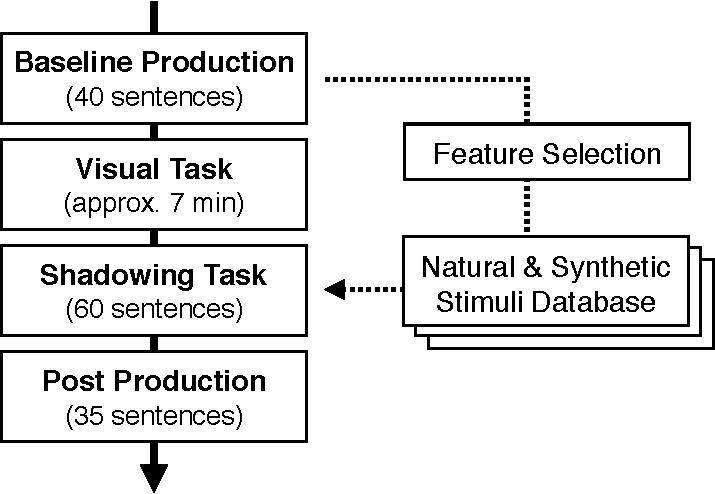
\includegraphics[width=\linewidth]{flow_experiment}
	\caption[\acs{hci} convergence experiment workflow]{Workflow of the experiment, showing its four phases. The stimuli presented in the shadowing task are selected based on feature realization in the baseline production.}
	\label{fig:HCIConvFlow}
\end{figure}

The experiment was carried out in a sound-proof booth located inside a recording studio.
Seeing that the experiment dealt with the way people change their way of speaking based on speech of others, conversation with participants was generally kept as minimal as possible.
It goes without saying, however, that it was not realistic to try and control for any kind of conversation the participants might have had during the day prior to the experiment.

In the first phase of the experiment, the base natural production of the participants was observed.
No instructions whatsoever were given regarding how they should speak.
An overview of the workflow in presented in~\autoref{fig:HCIConvFlow}.
The participants were to read 40 sentences from a monitor.
\review{explain fillers etc.}
The sentences were all in grammatical German and relatively short (5-7 words), with some being declarative and some interrogative.
No signal was introduced to tell the participants to start reading (aside from the sentence to appear on the monitor after a blank \enquote{pause} screen), and the average pausing time between uttering two sentences was
\todo{insert time}
milliseconds.
Utterances of sentences containing a target feature were examined on-the-fly, and the way they were produced by the participant was marked.

The second phase was a short pause, about seven minutes long.
Its purpose was to let the mental representation of the production to fade, so that the base production will not influence as much on the productions in the following parts.
To boost this process, the participants played a game with strong visual aspects and with non-verbal sounds only.
Conversing with the participant was avoided as much possible as possible in order to prevent from other verbal input to influence their mental representations.
The participants' performance in the game was not recorded and did not influence the next parts in any way.

The third phase

The fourth and final phase

A Java-based program with \ac{gui} was developed exclusively for this experiment.
Its functionality was tailored for the setup and the phases described above.
This includes test sentences for setting up output volumes (participant's headset, experimenters' speaker, etc.), auto shuffling the stimuli into a balanced list, convenient way of choosing the correct stimuli from the database (correct set plus considering the participant's pronunciation preferences), logging the times and stimulus order, playing and replaying stimuli, and more.
\review{want to upload this program and give a link here?}

\subsection{Results}
\label{subsec:results_hci}

\begin{figure}[!t]
	\centering
	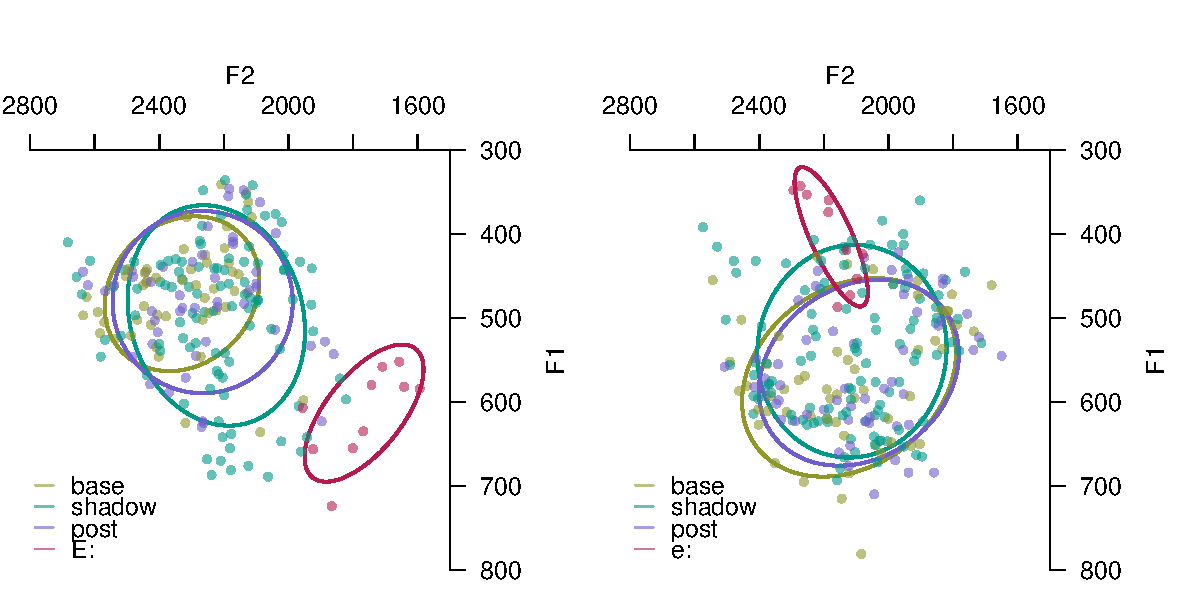
\includegraphics[width=\textwidth]{formant-plot}
	\caption[short caption]{long caption}
	\label{fig:HCIConvFormants}
\end{figure}

\fixme{how to put schwa and ic-ik next to each other?}

\begin{figure}[!t]
	\centering
	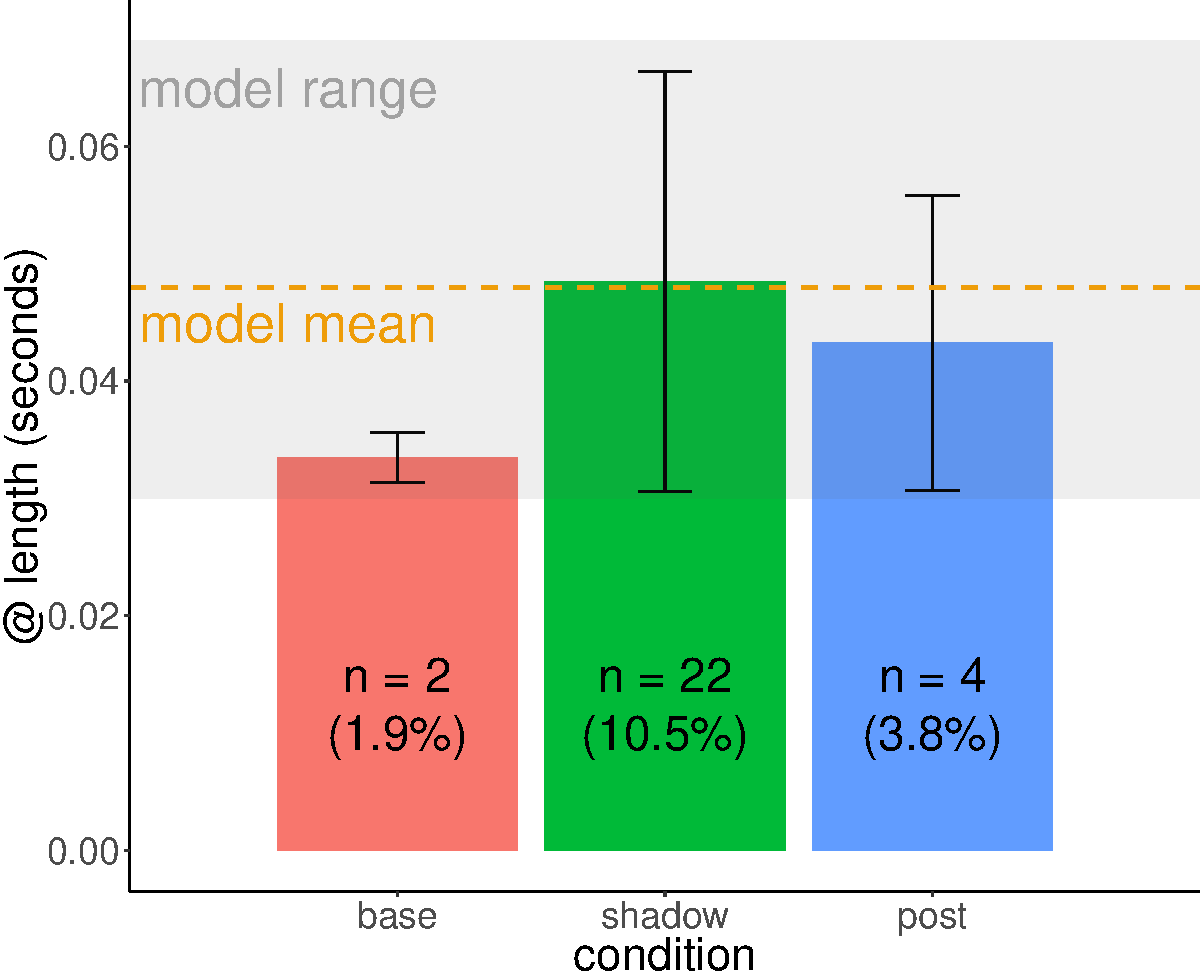
\includegraphics[width=0.5\textwidth]{schwa-plot}
	\caption[short caption]{long caption}
	\label{fig:HCIConvSchwaPlot}
\end{figure}

\begin{figure}[!t]
	\centering
	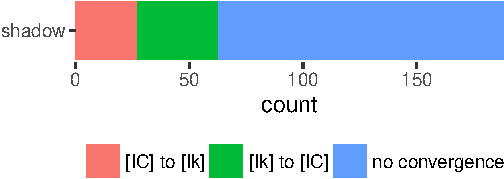
\includegraphics[width=0.5\textwidth]{ich_ik-plot}
	\caption[short caption]{long caption2}
	\label{fig:HCIConvIcIkPlot}
\end{figure}

\subsection{Generation of the synthetic stimuli}
\label{subsec:generation_stimuli_hci}

After finding some convergence effect to the natural stimuli, the next step is to test whether the same convergence effect is present also occurs when presenting synthetic stimuli to the participants.
For that, synthetic (i.e.\ computer generated) stimuli need to be created.
There are multiple methods to synthesize speech:
formant synthesis \citep[e.g.][]{Burkhardt2000verification}, unit selection \citep{Hunt1996unit,Black2003unit}), diphone synthesis \citep{Dutoit1996mbrola}, and probabilistic (e.g., using \acp{hmm} as described in \citet{Zen2005overview} and in \citet{Zen2009statistical}), to name some.

Seeing that the experiment in question examines convergence in specific segment-level phonetic features, it is preferable to fix other speech characteristics like intonation and stress, in order to prevent from those to influence the perception of the sentences by the listeners.
To achieve that, the f$_0$ contours and segment durations of the natural stimuli were imposed on the synthetic stimuli.
These values were extracted from the annotations of the natural stimuli (see \citet{Gessinger2016PundP}):
The segment durations were directly taken from the annotations, and the f$_0$ contours were acquired by first interpolating the contour of the natural stimuli, and then record the f$_0$ value at the beginning and at the middle of each segment.
These two values per segment were used in the synthesis.
It goes without saying, however, that the generated contours were not \emph{completely} identical to those of the corresponding natural stimuli, but no substantial differences in overall sentence intonation or stress were introduced.
